\documentclass[10pt,landscape]{article}
\usepackage[utf8]{inputenc}
\usepackage{multicol}
\usepackage{calc}
\usepackage{ifthen}
\usepackage[landscape]{geometry}
\usepackage{hyperref}
\usepackage{amsmath, amssymb, amsthm, bm, hyperref, float}
% \usepackage{minted}
\usepackage{graphicx}
\usepackage{mathtools}
\usepackage{caption, subcaption}
\DeclarePairedDelimiter{\ceil}{\lceil}{\rceil}
\graphicspath{{images/}}

% This sets page margins to .5 inch if using letter paper, and to 1cm
% if using A4 paper. (This probably isn't strictly necessary.)
% If using another size paper, use default 1cm margins.
\ifthenelse{\lengthtest { \paperwidth = 11in}}
    { \geometry{top=.5in,left=.5in,right=.5in,bottom=.5in} }
    {\ifthenelse{ \lengthtest{ \paperwidth = 297mm}}
        {\geometry{top=1cm,left=1cm,right=1cm,bottom=1cm} }
        {\geometry{top=1cm,left=1cm,right=1cm,bottom=1cm} }
    }

% Turn off header and footer
\pagestyle{empty}


% Redefine section commands to use less space
\makeatletter
\renewcommand{\section}{\@startsection{section}{1}{0mm}%
                                {-1ex plus -.5ex minus -.2ex}%
                                {0.5ex plus .2ex}%x
                                {\normalfont\large\bfseries}}
\renewcommand{\subsection}{\@startsection{subsection}{2}{0mm}%
                                {-1explus -.5ex minus -.2ex}%
                                {0.5ex plus .2ex}%
                                {\normalfont\normalsize\bfseries}}
\renewcommand{\subsubsection}{\@startsection{subsubsection}{3}{0mm}%
                                {-1ex plus -.5ex minus -.2ex}%
                                {1ex plus .2ex}%
                                {\normalfont\small\bfseries}}
\makeatother

% Define BibTeX command
\def\BibTeX{{\rm B\kern-.05em{\sc i\kern-.025em b}\kern-.08em
    T\kern-.1667em\lower.7ex\hbox{E}\kern-.125emX}}

% Don't print section numbers
\setcounter{secnumdepth}{0}


\setlength{\parindent}{0pt}
\setlength{\parskip}{0pt plus 0.5ex}


% -----------------------------------------------------------------------

\begin{document}

\raggedright
\footnotesize
\begin{multicols}{3}


% multicol parameters
% These lengths are set only within the two main columns
%\setlength{\columnseprule}{0.25pt}
\setlength{\premulticols}{1pt}
\setlength{\postmulticols}{1pt}
\setlength{\multicolsep}{1pt}
\setlength{\columnsep}{2pt}

% =============================================================================

\section{Out-of-Core Algorithms}

\textbf{Map}: Read a batch to an input buffer, process it, write to an output buffer. When input buffer consumed, read more data in; when output buffer consumed, write to disk \\
\textbf{Rendevous}: Can't keep everything in memory, so make sure codependent items appear in memory at the same time (\textit{time-space rendevous}) \\

\textbf{2-Way External Mergesort}

\begin{itemize}
    \item Pass 0 (Conquer): Read a page, sort it, write it to disk. Only one buffer page used.
    \item Pass $>0$ (Merge): Requires 3 buffer pages (2 input, one output). Merges pairs of runs into runs twice as long.
    \item Total cost: $2N(\ceil*{log_2 N} + 1)$
\end{itemize}


\textbf{External Mergesort}

\begin{itemize}
    \item Pass 0 (Conquer): Use $B$ buffer pages and produce $\ceil*{N/B}$ sorted runs of $B$ pages each
    \item Pass $>0$ (Merge): Merge $B-1$ runs at a time
    \item \# of passes: $1+\ceil*{\log_{B-1}\ceil*{N/B}}$
    \item Total cost: $2N * (\# of passes)$
    \item Can sort $B(B-1)$ pages in 2 passes
\end{itemize}

\textbf{Internal Sort}

Heapsort: Keep two heaps $H1$ and $H2$ in memory, read $B-2$ pages and insert into $H1$. Drain $H1$ with variable $m$ and place new records $<m$ into $H2$ and larger entries into $H1$. When $H2$ fully drained, swap $H1$ into $H2$ and repeat until there are no more records. Average run length is $2(B-2)$.

\textbf{Hashing}

Many operations don't require order, so sorting is unnecessary. Use hashing to rendevous matches. $4*N$ I/Os.

\textit{Divide}: Use a hash function to stream records to disk partitions \\
\textit{Conquer}: Rehash partitions into RAM partitions using a different hashing function

\textit{Recursive Partitioning}: If disk partition too big after pass 0, divide partition using a different hash function.

% =============================================================================

\section{SQL}

% \begin{verbatim}
% SELECT [DISTINCT] target-list
% FROM relation-list
% WHERE qualification
% GROUP BY grouping-list
% HAVING group-qualification
% \end{verbatim}
%
% \textbf{Useful keywords}
%
% \begin{verbatim}
% INTERSECT
% JOIN...ON...
% (NOT) IN
% \end{verbatim}

\textbf{Inner/Natural join}: equi-join for each pair of attributes with the same name \\
\textbf{Left outer join}: Returns all matched rows and all unmatched rows from table on left \\
\textbf{Right outer join}: Returns all matched rows and all unmatched rows from table on right \\
\textbf{Full outer join}: Returns all matched and unmatched rows. Unmatched rows from one side have \texttt{NULL} for attributes on the other side.

\textbf{Integrity Constraints}: conditions that every legal instance of a relation must satisfy (e.g. domain/primary key/foreign key/general constraints) \\
\textbf{Keys}: Primary (at most one), candidate (unique), foreign (referential integrity, no dangling references)

% \textbf{Median}
%
% (Assumes T has an odd number of rows):
%
% \begin{verbatim}
% SELECT c AS median FROM T
% WHERE
%     (SELECT COUNT(*) from T AS T1
%         WHERE T1.c <= T.c)
%     =
%     (SELECT COUNT(*) from T AS T2
%         WHERE T2.c >= T.c);
% \end{verbatim}
%
% Works for any number of rows:
%
% \begin{verbatim}
% SELECT x.c as median
% FROM T x, T y
% GROUP BY x.c
% HAVING
%     SUM(CASE WHEN y.c <= x.c THEN 1 ELSE 0 END)
%         >= (COUNT(*)+1)/2 -- ceil(N/2)
% AND SUM(CASE WHEN y.c >= x.c THEN 1 ELSE 0 END)
% \end{verbatim}

% =============================================================================

\section{Disk Layout}

\textbf{Page}: Tables stored as logical files consisting of \textit{pages} of \textit{records}. Pages in managed in memory by buffer manager, on disk by disk space manager. \\
\textbf{LRU}: Works well for repeated accesses to popular pages (temporal locality). Costly, needs to maintain heap structure. \\
\textbf{MRU}: Best for repeated scan of big file (fixes sequential flooding) \\
\textbf{Clock Replacement}: Arrange frames in cycle with ref bit, "second chance LRU"

Best for DBMS to handle page/buffer management over OS because DBMS requires page pinning and flushing pages to disk, which is important for implement CC and recovery. In addition, the DBMS can adjust the replacement policy and prefetch pages based on access patterns in typical DB operations.

\begin{tabular}{@{}ll@{}}
Unordered heap      & records placed on arbitrary pages \\
Clustered heap/Hash & records/pages grouped \\
Sorted files        & pages/records in sorted order \\
Index files         & B+ trees, hash tables
\end{tabular}

\textbf{Files}: Higher levels of DBMS operate on pages of records and files of pages. File must support insert/modify/delete record, fetching record by record id, scanning all records. Can span multiple machines/OSes. \\
\textbf{Page header}: Contains number of records, free space, next/last pointer, slot table \\
\textbf{Fixed-length records}: \textit{Packed}: pack records densely, record record id in page, append on add, rearrange on delete. \textit{Unpacked}: header contains bitmap of filled slots; on insert fill first empty slot, on delete clear bit. \\
\textbf{Slotted page}: Slot directory in header, each slot has length of record and pointer to the beginning of the record; header has number of slots and pointer to free space. Delete sets pointers to \texttt{NULL}; insert into first large-enough slot. Grow records from end of page so slot directory can be extended on insert. On insert, extend slot directory, add record in free space, update slot counter in header. \\
\textbf{Record formats}: Assume system catalog with schema (no need to store type information, format stored in another table). For variable length, record header stores pointers to ends of variable-length fields. Also covers NULL fields, useful for fixed-length.

% =============================================================================

\section{Join Operators}

\textbf{Cost notation}:

\begin{tabular}{@{}ll@{}}
$[R]$   & \# pages to store $R$ \\
$p_R$   & \# records per page of $R$ \\
$|R|$   & cardinality of $R$ (\# records)
\end{tabular}

Assume in join $R$ is left, $S$ is right, can be swapped if necessary. Assume we have $B$ pages of memory.

\textbf{Costs}

\textit{Simple nested-loop}: For each record in $R$, loop through each record in $S$ and compare. Cost: $(p_R \times [R]) \times [S] + [R]$

\textit{Page-oriented nested-loop}: Same as before, but for each page in $R$, loop through each page in $S$. Cost: $[R] \times [S] + [R]$

\textit{Block nested-loop}: Same as before, but for each block in $R$ of size $B-2$, loop through each page in $S$. Cost: $[S]\times\ceil*{[R] / (B-2)} + [R]$. Use when join condition doesn't filter many rows or one table fits in a small number of memory blocks.

\textit{Index nested-loop}: For each tuple in $R$, lookup $r_i$ in index on $S$. Cost: $[R] + ([R] \times p_R) \times \text{lookup time for index on S}$

\textit{Grace Hash join}: Partition $R$ and $S$ by hashed join key and write to disk. Use new hash function to build size $B-2$ hash table of elements from smaller table (say $R$), then load each page from $S$ and probe. Cost: $3([R]+[S])$; $N$ if each table has $\le B$ pages, $3N$ if $B < n \le B^2$. serial I/O, so no seek overhead. Use if one table fits into memory, or if we can use hybrid hashing.

\textit{Sort-merge}: Sort both $R$ and $S$. Walk through both $R$ and $S$ in sequence and probe. Cost: $Sort(R) + Sort(S) + ([R] + [S])$, last term could be $[R] \times [S]$ worst case. Refinement: do join during final merging pass of sort; Cost: $3[R] + 3[S]$. Especially good choice if one or both inputs sorted on join attributes, output required to be sorted on join attribute, input data is skewed and hash join could lead to recursive partitioning, number of pages in memory is small.

\textit{Hybrid hashing}: Refinement of Grace hash join to take advantage of more memory. Hold partition 0 in memory instead of writing to disks; saves I/Os.

% =============================================================================

\section{Tree Indexes}

Data structure that enables fast lookup of data entries by search key

\textbf{Alternatives}

\begin{tabular}{@{}ll@{}}
A1 & By value, entire record in leaf \\
A2 & By reference, (key, rid)\\
A3 & By list of refs, (key, [rid]) \\
\end{tabular}

\textit{Clustered index}: Index whose search key specifies the sequential ordering of the file \\
\textit{Unclustered index}: Table file not ordered by unclustered index field; range lookups much slower \\
\textit{Multiple indexes}: Constructed on different individual columns \\
\textit{Multi-column index}: Constructed on concatenated columns \\


\subsection{Indexed Sequential Access Method (ISAM)}

Static structure! \\
\textit{File creation}: Leaf (data) pages stored in order by search key, then index pages, then overflow pages \\
\textit{Search}: start at root, use key comparisons to go to leaf \\
\textit{Invariant}: With a node $[..., (K_L, P_L), (K_R, P_R), ...]$, all tuples in range $K_L \le K < K_R$ are in tree $P_L$ \\
\textit{Complexity}: $\mathcal{O}(\log_F(\# pages))$ \\
\textit{Insert}: Find leaf that data entry belongs to and add it. Create overflow page if necessary, and link to leaf page with double pointers.
\textit{Delete}: Find entry in leaf and delete it. If deleting tuple empties overflow page, deallocate it and remove from linked list.

Pros: Sequential storage, scan all records without touching index. Good for static data setting with big scans. Cons: Doesn't handle insertion/deletion well, degrades to linear search.

\subsection{B+ tree}

\textit{Occupancy invariant}: Each interior node is partly full ($d \le \# entries \le 2d$), where $d$ is the order of the tree (max fan-out = $2d + 1$)

Order makes little sense with variable-length entries (e.g. single entry fills entire page, different nodes have different number of entries). Use physical criterion - at least half-full; many real systems only reclaim space when page completely empty (reduces I/Os).

Data pages at bottom not in sequential order, require next/last pointers \\
Typical order 1600, fill factor 67\%. Levels 1 and 2 can usually be stored in buffer pool.

\textit{Search}: Binary search on each page for node split, follow pointer to next node \\
\textit{Insertion}: Search for correct leaf, add entry if page not full, sort if necessary. If not enough space, split leaf and redistribute entries evenly (new entry goes on right side of split). Copy up middle key and recursively split index nodes, pushing up middle key each time \\
\textit{Bulk-Loading}: Sort input records by key, fill leaf pages to fill-factor and keep updating parent until full. Split parent by pushing all entries to sibling to achieve fill factor, push one entry to parent to combine node and sibling. Occupancy invariant not held on right branch. \\
\textit{Suffix key compression}: Increases fan-out by moving common prefix to header.

% =============================================================================

\section{Relational Operators}

One-to-one relationship between SQL query and relational algebra; SQL is declarative expression of query result, relational algebra is operational description of a computation

Pure relational algebra has \textit{set semantics}, but relaxed for system discussion

\textit{Closed}: result is also a relational instance, enables composition \\
\textit{Typed}: input schema determines output

\textbf{Unary operators}:

\begin{tabular}{@{}ll@{}}
$\pi_{cols}(In)$                        & projection \\
$\sigma_{condition}(In)$                & selection \\
$\rho(Out(old \rightarrow new), In)$    & renaming
\end{tabular}

\textbf{Binary operators}:

\begin{tabular}{@{}ll@{}}
$\cup$                      & \texttt{UNION} \\
$\cap$                      & \texttt{INTERSECT} \\
$-$                         & set difference, \texttt{EXCEPT} \\
$\times$                    & cross product \\
$\bowtie_\Theta, \bowtie$   & join
\end{tabular}

\textbf{Monotonicity}: If not monotone, operation is blocking. Relational operator $Q$ is monotone in $R$ if

\begin{equation}
    R_1 \subseteq R_2 \rightarrow Q(R_1, S, T, \ldots) \subseteq Q(R_2, S, T, \ldots)
\end{equation}

Implementing intersect with set difference: $S1 \cap S2  = S1 - (S1 - S2)$ \\
Hierarchy: Theta join $\rightarrow$ Equi-join $\rightarrow$ Natural join

% =============================================================================

\section{Query Optimization}

\textit{System R query optimization}: Left-deep only, avoid cross-products, push selections/projections down. Interesting orders: ORDER BY, GROUP BY, downstream join attributes \\
\textit{Selectivity (RF) estimation}: $\frac{|output|}{|input|}$.

\begin{itemize}
  \item If col = value, $RF = 1 / NKeys(R)$
  \item If col1 = col2, $RF = 1 / max(NKeys(R1), NKeys(R2))$
  \item If col $>$ value, $RF = (High(R)-value) / (High(R) - Low(R) + 1)$
\end{itemize}

\textit{Assumptions}: Values are uniformly distributed and terms are independent. If missing required statistics, use $1/10$. \\
\textit{Histograms}: For better estimation on statistics, use a histogram. Equiwidth, equidepth, v-optimal


\textit{Single table cost estimation}: Sequential scan: $NPages(r)$. \\
Equality selection on key of index $T$: $Height(T) + 1$ \\
Selections on clustered index T: $(NPages(T) + NPages(R)) \prod RFs$. \\
Selections on unclustered index T: $(NPages(T) + NTuples(R)) \prod RFs$.

% =============================================================================

\section{Concurrency}

\textit{Atomicity}: All or none of the actions in xact happen \\
\textit{Consistency}: DB must be consistent before/after xact. Expressed as series of integrity constraints (CREATE TABLE/ASSERTION statements) \\
\textit{Isolation}: Effects of one xact are isolated from those of others. \\
\textit{Durability}: If xact commits, its effects persist.

Transaction either commits or aborts (or system crash during xact, treat as abort). Logging: undo actions of aborted/failed xacts, redo actions of committed xacts when system crashes.

\textit{Serial schedule}: Xact runs from start to finish without intervening actions from other xacts. \\
\textit{Equivalent}: Involve some actions of same xacts, leave DB in same state \\
\textit{Conflict equivalent}: involve same actions of same transactions, every pair of conflicting actions ordered the same way \\
\textit{View serializability}: Same initial reads: $T_i$ reads initial value of A in $S_1$, then $T_i$ also reads initial value of A in $S_2$. Same dependent reads: If $T_i$ reads value of A written by $T_j$ in $S_1$, then $T_i$ also reads value of A written by $T_j$ in $S_2$. Same winning writes: If $T_i$ writes final value of A in $S_1$, then $T_i$ also writes final value of A in $S_2$. \\
\textit{Dependency graph}: One node per xact, edge from $T_i$ to $T_j$ if an earlier operation of $T_i$ conflicts with an operation of $T_j$. Conflict-serializable iff dependency graph is acyclic \\
\textit{Waits-for graph}: Edge from $T_i$ to $T_j$ means that $T_j$ is holding a resource that $T_i$ needs, and $T_i$ is waiting on $T_j$. Periodically check for cycles in the graph and kill a transaction in the cycle. \\
\textit{Two-phase locking}: xact must get a shared lock before reading, exclusive lock before writing. Cannot get new locks after releasing any locks. Does not prevent cascading aborts. \\
\textit{Strict 2PL}: Locks released only when xact completes (commit or abort). Prevents cascading aborts. \\
\textit{Lock manager}: handles lock/release requests. Keeps an entry for each key: (holders, waiters, shared/exclusive). \\
\textit{Deadlock}: Deal with by prevention, avoidance, detection, use timeout. \\
\textit{Deadlock avoidance}: Wait-die: If $T_i$ higher priority, $T_i$ waits for $T_j$ else $T_i$ aborts. Wound-wait: If $T_i$ higher priority, $T_j$ aborts else $T_i$ waits. Priority usually based on transaction's age. Make sure if transaction restarts, it gets its old timestamp. \\
\textit{Granularity}: database $\rightarrow$ tables $\rightarrow$ pages $\rightarrow$ tuples \\
\textit{Intent locks}: IS, IX, SIX. To get S or IS, must hold IS or IX on parent. To get X or IX or SIX, mut hold IX or SIX on parent. Must release locks in bottom-up order.


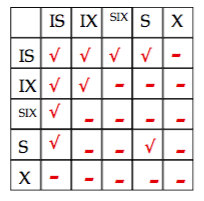
\includegraphics[width=.3\linewidth]{lock_compat.png} \hfill 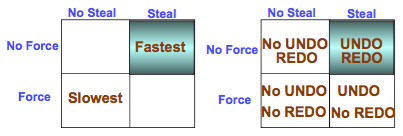
\includegraphics[width=.65\linewidth]{force_steal.png}

% =============================================================================

\section{Recovery}

\centerline{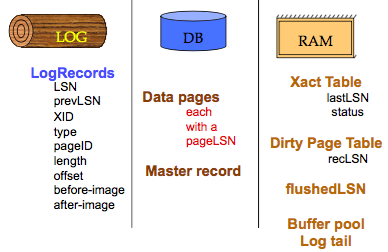
\includegraphics[width=.6\linewidth]{log_loc.png}}

\textit{Recovery manager}: ensures atomicity and durability (also consistency-related rollbacks) \\
\textit{Force policy}: make sure every update on DB disk before committing, slow. No-force: allow commits without flushing dirty pages to disk \\
\textit{No steal policy}: Don't allow buffer-pool frames with uncommitted updates to overwrite committed data on disk, slow. Steal policy: system can evict/flush pages with uncommitted udpates. \\
\textit{Logging}: REDO/UNDO action pairs. (XID, pageID, offset, length, old data, new data). Possible log record types: update, commit, abort, checkpoint (for log maintenance), compensation log records (CLR) for UNDO, END (commit or abort). \\
\textit{Log sequence number (LSN)}: always increasing. Each data page contains a pageLSN, LSN of most recent log record for update to that page. System keeps track of flushedLSN, max LSN flushed so far. \\
\textit{Write-ahead logging}: Force the log record for an update before the corresponding data page gets to disk. Force all log records for xact before commit. Before page i is written to DB, $pageLSN_i < flushedLSN$. \\
\textit{Transaction table}: one entry per xact: (XID, status (run/commit/abort), lastLSN (most recent LSN written by xact)). \\
\textit{Dirty page table}: one entry per dirty page in buffer pool. Contains recLSN (LSN of log record which first caused page to become dirty). \\
\textit{Transaction abort}: Get lastLSN of xact from xact table. Write new abort log record at end of log before beginning rollback. Follow chain of log records backwards via prevLSN. Write CLR for each undone operation.

\subsection{Crash Recovery}

\textit{Analysis}: Start at last checkpoint. Re-establish knowledge of state at checkpoint via transaction table and dirty page table stored in checkpoint. Scan log forward from checkpoint. End record: remove xact from xact table 9done). Other records add xact to xact table, set lastLSN = LSN, change xact status on commit. For update records: if P not in dirty page table, add P to DPT, set recLSN = LSN. recLSN is first LSN that caused page to become dirty. At end of analysis, xact table says which xacts were active at last log flush before crash. DPT says which dirty pages might not have made it to disk. \\
\textit{Redo}: Repeat history to reconstruct state at crash. Reapply all updates (even of aborted xacts), redo CLRs. Scan forward from log rec containing smallest recLSN in DPT. For each update log/CLR with given LSN, redo unless: (Affected page not in DPT, affected page in DPT but $recLSN > LSN$, $pageLSN(inDB) \ge LSN$ (slow!)). For each redo action, reapply logged action and set pageLSN to LSN. No additional logging/forcing. At end of redo phase, end type records are written for all transactions with committed status. \\
\textit{Undo}: Effects of failed xacts. Keep track of toUndo set: lastLSNs of all xacts in xact table. Repeat until toUndo is empty: Pop largest LSN among toUndo. If LSN is CLR and undoNextLSN = NULL: write END record for xact. If LSN is CLR and undoNextLSN $\ne$ NULL: Add undoNextLSN to toUndo. Else: LSN is an update. Undo update, write CLR, add prevLSN to toUndo. Lets us do one backwards pass of the log.

% =============================================================================

\section{Distributed Data}

\textit{2-phase commit}:

\begin{enumerate}
  \item Coordinator tells participants to prepare. Participants respond with yes/no votes. Must be unanimous to procede.
  \item Coordinator broadcasts either commit/abort depending on vote. Participants ack.
\end{enumerate}


% =============================================================================


\end{multicols}
\end{document}
